\chapter{绪论}
\section{研究背景及意义}
物联网(WoT)是W3C领导的一个重要趋势,旨在通过采用经过验证的Web技术来解决物联网(IoT)互操作性问题。
根据Gartner的分析,数十亿部署的物联网设备将产生泽字节(ZettaBytes, ZB)的数据。
随着WoT的发展趋势,可以预见,未来将有越来越多的数据集成到网络中。
对于如此大规模的数据,使用去中心化服务器(例如AWS IoT、阿里云等)来管理它会遇到单点故障等问题。
尽管分布式数据库可以避免单点故障,但由于数据安全性和不可篡改性较弱,在需要高度透明的情况下,它们很容易受到数据篡改攻击,例如物联网数据共享~\cite{chen2022blockchain}。

区块链以可追溯性和不变性为特征,可以解决集中式存储的单点故障问题和分布式数据库的恶意篡改问题。
它将数据存储在去中心化的账本中,并使用共识协议来解决平等节点之间的冲突,这种方式增强了安全性,提高了透明度,降低了成本,支持点对点协作。
尽管它具有巨大的潜力,但其较低的交易速度和较高的计算要求使其仅广泛应用于价值巨大但密度很低的领域,如金融服务、供应链管理等。

有许多研究人员致力于提高基于区块链的存储系统的性能。
根据数据的存储位置,这些工作可以分为两类,即链上存储和链下存储。
对于链上存储,数据作为存储在区块链上的交易记录的一部分,用户通过索引(即Merkle Patricia Trie,MPT)获取这些数据。
现有工作通过提供用户友好的查询语言~\cite{zhu2019sebdb,xu2019vchain,wang2022vchain+}提高了系统可用性,并通过改进索引方案~\cite{li2023lvmt,zhang2024cole}、区块链存储分片~\cite{zamani2018rapidchain,hong2023gridb,el2019blockchaindb}提高系统吞吐量。
然而,在链上存储物联网数据的开销非常高。
对于大量快速生成的物联网数据,将其连续存储在区块链上需要实现共识和分类账复制的过程,这可能会导致巨大的存储压力和通信开销。
因此,物联网数据存储的一种更实用的方法是利用链下存储解决方案。
对于链下存储,数据存储在区块链之外,区块链只存储必要的元数据或对数据的引用,如哈希或加密指针。
链下存储提供了比链上解决方案更大的可扩展性和更低的成本,因此业界和学术界对链下存储有很多兴奋,例如Storj~\cite{storj2018storj}、BigchainDB~\cite{mcconaghy2016bigchaindb}、Sia~\cite{sia}等。
然而,现有的作品大多是为存储大文件而设计的。
对于小型物联网数据,考虑到海量的物联网数据量,在区块链中存储每个数据项的哈希值将产生令人难以置信的开销。
此外,物联网应用场景通常需要存储系统支持高效查询(例如聚合查询),而现有的基于文件的存储系统不支持这一点。

\section{论文主要工作}
本文提出了一种高效的时间序列数据链下区块链存储系统TimeChain。
该系统对离散时间序列数据进行批处理,仅将每批数据的哈希值存储在链上,并将完整的原始数据保存在链外。
这种批处理存储方法大大减少了数据开销。
我们对链下区块链存储系统的性能进行了测量。
根据我们的测量,与单个数据存储相比,存储延迟平均减少了37.4倍。
这种存储性能使基于区块链的时间序列数据存储成为可能。

然而,不可否认的是,这也会影响查询性能。
具体来说,当用户执行聚合查询时,低效的批处理方法会导致在多个传输节点上获取数据,从而导致额外的传输延迟。
此外,由于区块链上只存储了批次的哈希值,因此存储系统必须传输额外的信息(例如Merkle树的哈希路径),以支持数据所有者执行数据完整性验证。
这进一步增加了查询开销。

为了减少范围查询过程中跨越的存储节点数量,我们提出了一种新的自适应打包机制。
我们通过从原始数据构建无向加权图,将批处理问题转化为图划分问题。
我们使用谱聚类算法通过将频繁查询的数据分组在一起来解决分区问题,以减少聚合查询期间的节点访问次数。

为了在确保系统安全的同时进一步减少查询延迟,我们提出了一种基于共识的存储节点选择机制。
在选择节点时,我们同时考虑存储节点信誉和传输距离。
为了在基于区块链的存储系统中快速做出节点选择决策,我们将共识过程与节点相结合,以减少传播延迟。

为了减少验证过程中的传输开销,我们提出了一种基于位置敏感散列(LSH)的数据完整性验证机制。
该机制基于相邻时间序列数据点之间的相似性,仅传输证明的非冗余部分,从而显著减少了完整性验证所需的数据。

我们基于生产就绪的开源组件(如Hyperledger Fabric和IPFS)实现TimeChain,并评估TimeChain的性能。
结果表明,与现有的基于区块链的存储系统相比,TimeChain平均减少了64.6\%的查询延迟和35.3\%的存储延迟。

\section{全文结构}
\section{本章小结}

\chapter{相关工作}

\section{区块链存储系统}
\subsection{分布式存储系统}
近年来,由于集中式数据存储解决方案的固有漏洞,特别是其易受单点故障的影响,分布式数据库越来越受到重视。
Apache Cassandra、Spanner和CockroachDB都是分布式键值存储系统,通过特殊的数据分发策略确保数据存储的高可用性和容错性。
然而,这些分布式存储系统仍然存在单点故障和高存储成本的问题。
即使数据已经分发到多个存储节点,数据的控制权仍然掌握在数据库供应商手中,这使得存储系统公司很容易在数据所有者不知情的情况下篡改数据。

\subsection{区块链存储系统}
目前,许多研究都集中在链上数据存储的性能上,包括查询性能和存储负担。
SEBDB~\cite{zhu2019sebdb}和MSTDB~\cite{zhou2022mstdb}通过引入不同的索引机制来实现这一点,以支持各种类型的查询,如类SQL查询和基于语义的多关键字查询。
与建立块级索引不同,LVMT~\cite{li2023lvmt}和COLE~\cite{zhang2024cole}优化了Merkle Patricia Trie上的索引,以提高区块链状态的查询速度。
为了减轻在分类账中存储数据的负担,Rapidchain~\cite{zamani2018rapidchain}、SlimChain~\cite{xu2021slimchain}和GriDB~\cite{hong2023gridb}将分类账分配给其他分片进行存储,以减轻存储压力。
TimeChain可以很容易地与这些链上存储优化解决方案相结合,以加速链上哈希的获取。
然而,在数据量大、生成快的物联网场景中,这些解决方案不仅带来了数据隐私泄露的风险,还给区块链带来了额外的空间存储负担,这不适合数据生成快的IoT场景。

\subsection{基于区块链的文件系统}
基于区块链的文件系统因其对文件完整性的保证而受到了广泛的研究和关注。
Filecoin~\cite{bauer2022filecoin}是一个基于IPFS~\cite{benet2014ipfs}的去中心化文件存储系统,它通过激励机制鼓励用户提供存储服务。
Storj~\cite{storj2018storj}和Sia~\cite{vorick2014sia}以半分散的方式为每个文件建立Merkle树,以确保文件完整性。
FileDES~\cite{xu2024filedes}专注于数据的加密存储。
它通过引入零知识证明等技术来保护数据存储的安全性。
然而,这些方法都不能提供高效的物联网数据存储。
由于物联网数据的价值密度较低,如果将单个数据以文件的形式存储在区块链文件系统中,将带来非常高的成本。

\section{移动区块链激励系统}

\chapter{面向物联网的高效区块链存储系统}

\section{需求和挑战}
\label{sec:baseline}
为了提高基于区块链的分布式数据库的性能,我们提出了一种基本的链下存储系统,并对其进行了测量研究。

\subsection{基于区块链的存储系统架构}

\begin{figure}[t]
    \centering
    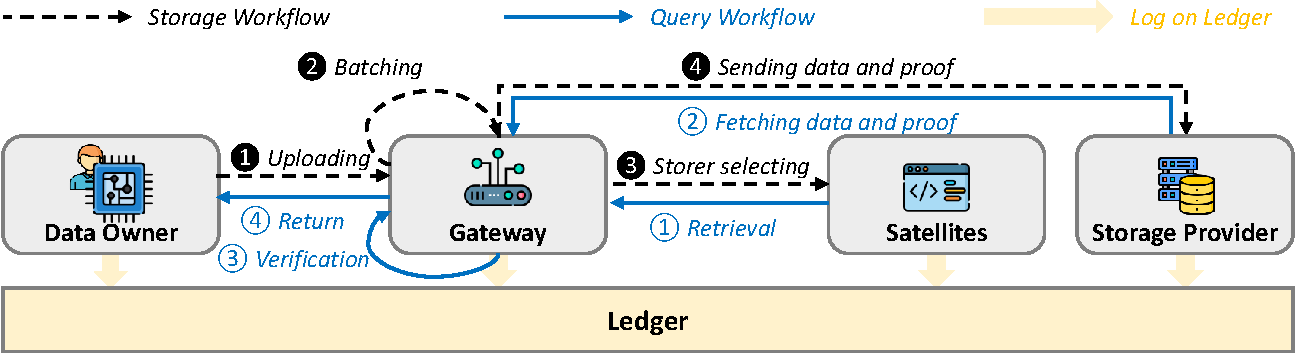
\includegraphics[width=1\linewidth]{timechain/measurement_workflow.pdf}
    \caption{基于区块链的存储系统的工作流}
    \label{fig:workflow}
\end{figure}

如~\autoref{fig:workflow}所示,一个基于区块链的基本分布式存储系统有四个主要角色,即数据所有者、网关、卫星和存储提供商。
数据所有者请求存储资源并查询数据。
网关为消费者提供了一个与网络交互的接口,允许他们上传、下载和管理数据。
卫星协调业主和供应商之间的沟通。
它们提供文件审计(Audit)或POR(可检索性)相关功能和存储支付处理。
为了确保过程的安全性,卫星通常以智能合约的形式运行。
存储提供商存储和检索数据,通过提供存储和带宽资源来获得奖励。
为了使存储提供商能够通过灵活的查询快速向数据所有者提供完整性证明,证明数据也需要存储在存储提供商中。
存储提供商的服务信息,如剩余存储空间,将与交互记录一起记录在分布式账本中,以确保安全。
一般来说,数据存储和查询过程可以概括如下:

\textbf{数据存储:}
\ding{182}\textit{正在上传}:
数据所有者通过网关接口上传数据。
\ding{183}\textit{批处理}:
网关对时间序列数据进行批处理,并生成每批数据的数据完整性证明。
\ding{184}\textit{存储选择}:
卫星帮助网关发现用于存储数据的最佳存储节点。
\ding{185}\textit{发送数据和证明}:
原始传感器数据和完整性证明被发送到最佳存储提供商。
数据批的元数据记录在分布式账本中。

\textbf{数据查询:}
\ding{172}\textit{检索}:
数据所有者请求下载他们的数据,网关与卫星交互以检索相应存储提供商的位置。
\ding{173}\textit{获取数据和证明}:
网关从存储提供商处获取数据和完整性证明。
\ding{174}\textit{验证}:
网关通过检查数据完整性证明来验证下载数据的完整性。
\ding{175}\textit{返回}:
网关将数据返回给数据所有者。

\subsection{基本架构测量研究}
在本节中,我们进行了一项初步研究,以评估基于区块链的基本存储系统的性能。
我们实现了基于Hyperledger Fabric的存储系统。
该测试网络由5个节点组成,其中1个节点既是网关,4个节点是卫星。
我们模拟了全球320家存储提供商。
\begin{figure*}[t]
    \centering
    \begin{minipage}{0.8\linewidth}
	    \centering
        \subfloat[存储时延]{
            \centering
            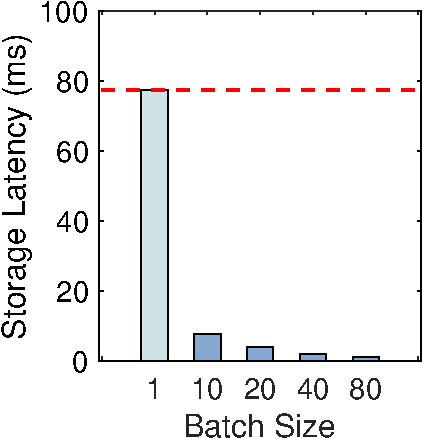
\includegraphics[width=0.45\textwidth]{timechain/measurement_storage.pdf}
            \label{fig:measurement_storage}
        }
        \hfill
        \subfloat[查询时延]{
            \centering
            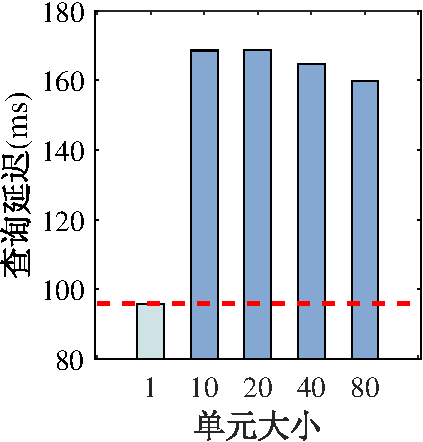
\includegraphics[width=0.45\textwidth]{timechain/measurement_query.pdf}
            \label{fig:measurement_query}
        }
        \caption{区块链存储系统的性能} 
    \end{minipage}
\end{figure*}

\textbf{存储性能。}
%我们将批次的大小设置为10。
我们设置数据所有者每秒生成20个56字节的数据包,并在20秒内存储它们。
存储性能结果如图所示。
与单独存储每个数据相比,批存储将延迟减少了约37.4倍。
这主要是因为较大的批处理规模减少了链上交易的数量。

\textbf{查询性能。}
然后,我们测试范围查询的性能,如图~\autoref{fig:measurement_query}所示。
不幸的是,结果显示,批处理存储解决方案的查询性能相对较差,在不同批处理大小下的平均延迟为165.4ms,无法满足许多物联网场景的需求。
例如,自动驾驶应用程序的延迟小于50ms,地震监测的延迟小于100ms。

\subsection{动机与挑战}
为了找出查询性能不佳的原因,我们进行了深入调查,并将原因总结为以下三点:

\begin{figure*}[t]
    \centering
    \begin{minipage}{1\linewidth}
	    \centering
        \subfloat[查询跨越多个batch]{
            \centering
            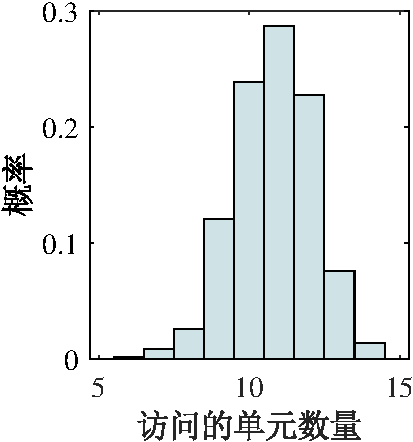
\includegraphics[width=0.3\textwidth]{timechain/batch_cdf.pdf}
            \label{fig:batch_cdf}
        }
        \hfill
        \subfloat[不正确的存储节点选择]{
            \centering
            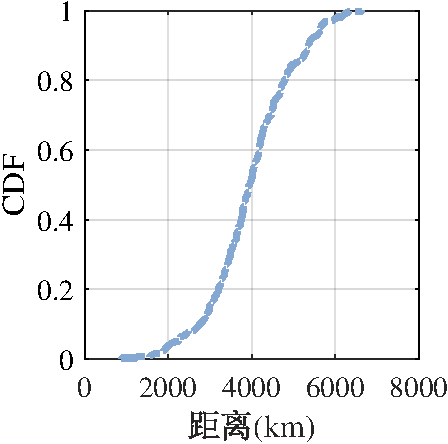
\includegraphics[width=0.3\textwidth]{timechain/dis_cdf.pdf}
            \label{fig:dis_cdf}
        }
        \hfill
        \subfloat[传输数据较大]{
            \centering
            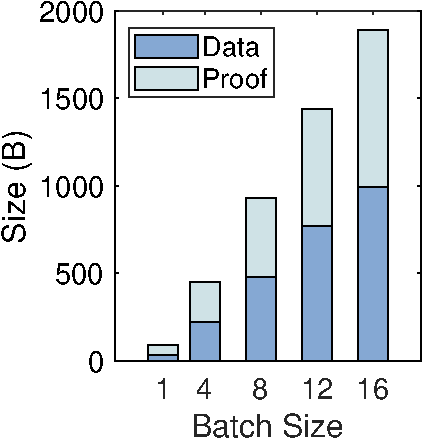
\includegraphics[width=0.3\textwidth]{timechain/proof_size_cdf.pdf}
            \label{fig:proof_size_cdf}
        }
        \caption{性能低下的根本原因} 
    \end{minipage}
\end{figure*}

\textbf{1)多个查询的生成批。}
时间序列数据的查询通常包含多个数据点,如范围查询、聚合查询、过滤查询等。
如果打包不当,单个查询可能会跨越多个批次。
我们使用现有的数据集YCSB~\cite{barata2014ycsb}评估每个查询所跨越的批次数量。
如图~\autoref{fig:batch_cdf}所示,超过84.25\%的查询跨越了10个批次。
当这些批驻留在不同的节点上时,会引入额外的查询和传输延迟。

\textbf{2)存储节点选择不当。}
在这个测量中,我们发现传输延迟占总查询延迟的很大一部分。
如图~\autoref{fig:dis_cdf}所示,世界各地存储节点的距离存在很大差异,导致节点之间的传输延迟存在很大差异。
如果选择非常远的存储节点,则会导致传输延迟增加。
此外,在存在恶意节点的情况下,存储节点的最终选择在传输延迟方面可能不是最优的,这会导致额外的传输开销。

\textbf{3)传输的证明文件大。}
为了使存储提供商能够通过灵活的查询快速向数据所有者提供完整性证明,证明数据也需要与存储提供商一起存储。
因此,当存储提供商需要向数据所有者证明数据的完整性时,数据证明也会被发送回数据所有者。
图~\autoref{fig:proof_size_cdf}显示了总传输数据的细分。
从图中可以看出,证明大小占接收数据的48.8\%,几乎是接收数据的一半。
当网络繁忙时,大量的证明会增加网络传输延迟。

\section{平台概览}
\label{sec:design}

\begin{figure}[t]
    \centering
    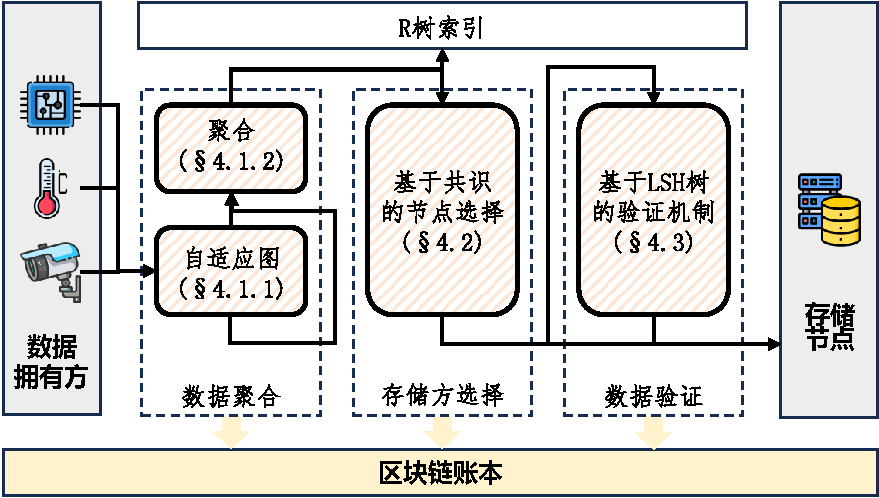
\includegraphics[width=1\linewidth]{timechain/arch.pdf}
    \caption{TimeChain架构}
    \label{fig:architecture}
\end{figure}

为了提高区块链存储系统的查询性能,我们设计了一种基于区块链的新型物联网时间序列数据存储系统TimeChain。
\autoref{fig:architecture}显示了TimeChain的架构。
TimeChain建立在区块链平台上,所有操作都记录在分布式账本上。
TimeChain中的核心模块包括数据批处理、存储器选择和数据验证。
TimeChain的索引结构是R树,可以加速物联网场景中常用的时空聚合搜索。
接下来,我们介绍TimeChain的关键模块。

\textbf{数据批处理模块:}
我们的测量研究表明,不正确的打包方法会增加查询的跨批数量,从而增加网络传输延迟。
我们构建了一个自适应无向加权图(UWG),以基于数据所有者的历史查询准确捕获用户查询信息(§-\ref{sec:UWG})。
对于我们构建的UWG,将哪些数据打包成批次的问题转换为聚类问题~\cite{xu2005survey},该问题根据用户的查询请求将所有原始数据划分为多个聚类。
解决聚类问题的传统算法有很多,如K-means~\cite{kanungo2002efficient}、GMM~\cite{he2010laplacian}等。
然而,这种传统的聚类算法不适合分割物联网设备生成的数据。
这是因为在TimeChain中,用户的查询没有遵循特定的特征,这可能会导致数据图的聚类形成复杂的形状,而不是常见的圆形。
此外,传统的聚类算法需要将所有数据划分为固定数量的集合,但并非所有集合都等于批大小,这将给索引查询带来额外的开销。
因此,我们使用谱聚类算法来打包数据(§-\ref{sec:ratiocut}),这非常适合处理不规则和非固定数量的聚类。

\textbf{存储节点选择模块:}
存储节点的\textit{选择}至关重要。
正如我们之前在图~\autoref{fig:dis_cdf}中发现的那样,存储节点和客户端之间的距离会影响数据访问延迟。
此外,对于链下存储数据库,存储空间不足的节点或恶意节点可能会导致数据丢失、篡改或服务中断,进而影响整个系统的安全性和稳定性。
因此,我们根据距离和历史服务记录等信息对存储节点进行综合评估。
存储节点\textit{选择过程的安全性}也非常重要。
Storj~\cite{storj2018storj}、CoopEdge~\cite{yuan2021coopedge}和PipeEdge~\cite{yuan2023pipeedge}通过一组固定的节点选择服务节点,并通过区块链确认决策。
换句话说,他们集中决策,但仍然面临单点失败的威胁。
然而,使用类似于PBFT的投票机制,节点选择过程通常需要多轮任务计算和消息广播。
如果共识过程和节点选择过程完全解耦,系统安全将受到威胁。
为了解决这个问题,我们将节点选择过程与共识相结合,提出了一种基于共识的节点选择机制(§-\ref{sec:consensus})。

\textbf{数据验证模块:}
从之前的测量结果中我们可以发现,传输的数据中有近一半是数据完整性证明。
数据证明被组织为Merkle树,它是由一系列哈希构建的。
在Merkle树中,非叶子节点的哈希数几乎等于原始数据点的数量。
由于物联网数据单元的大小大约等于哈希值,这意味着需要发送以验证数据的数据量几乎是原始数据的两倍。
减小数据证明的大小是一个挑战。
在分析物联网数据时,我们观察到物联网数据变化缓慢,在短时间内很少出现突然变化。
对于这些相似的数据,局部敏感哈希(LSH)算法可以从相似的原始数据中生成相似的哈希结果。
LSH确保类似的物联网数据即使在散列后也保持相似。
因此,我们提出了一种新的基于LSH树的验证机制(§-\ref{sec:LSH}),该机制采用LSH而不是传统Merkle树中使用的通用散列。
通过差分传输LSH哈希值,可以显著减小传输数据的大小。

\section{自适应聚合机制}
\label{sec:packaging}

对于数据打包,我们构建了一个基于历史查询的自适应UWG来表征动态查询范围。
通过运行自适应UWG的谱聚类算法,我们根据随机用户查询将原始数据打包成批。

\subsection{基于历史查询的自适应图}
\label{sec:UWG}

\begin{table}
    \centering
    \caption{符号表}
    \begin{tblr}{
      column{1} = {c},
      hline{1,13} = {-}{0.08em},
      hline{2} = {-}{0.05em},
    }
    \textbf{Symbol} & \textbf{Description}\\
        $d_i$   & The $i$th device \\
        $D$     & Set of the total devices, $D = \{d_0, ..., d_n\}$\\
        $s_i$   & The $i$th data generated by IoT sensors \\
        $S$     & Set of the total data, $S = \{s_0, ..., s_m \}$\\
        $Q^i$   & Set of $i$th user query, $Q^i = \{ q_0, ..., q_r \}$\\
        $q_k$   & The $k$th query in $Q^i$ \\
        $l_{ab}$& The weight of query contains device $a$ and device $b$ \\
        $L$     & The weight of data queried together, $L = \{l_{ab} | \exists_{a,b} \in D \}$\\
        $x^k_{ab}$ & Whether device $a$ and device $b$ are queried at the same time \\
        $X^k$   & The access information of devices, $X^k = \{x^k_{ab} | \exists_{a,b} \in D \}$\\
        $P$     & The data packaging result, $P = \{ \{ s_i, ... \}, ... \}$
    \end{tblr}
    \label{tab:notations}
\end{table}

由于物联网的原始数据是孤立的点,我们在数据点之间创建加权边,表示被联合查询的概率。
点$a$和$b$之间的边的权重表示为:

\begin{equation} 
    \label{eq:weight}
    \begin{split}
        l_{ab} =
        \begin{cases}
            \sqrt{ (id_a - id_b)^2 + (t_a - t_b)^2 } &, k = 0 \\  
            \theta \cdot l_{ab} + (1 - \theta) \cdot x_{ab}^k &, k \geq 1  
        \end{cases}
    \end{split}
\end{equation}

\subsection{基于谱聚类算法的封装机制}
\label{sec:ratiocut}
由于谱聚类算法适用于处理不规则形状的分类问题,我们使用它来打包数据。
\ref{algo:package}显示TimeChain的整个打包过程。
该算法的输入包括输入设备集$D$、数据集$S$和用户的历史查询集$Q^i$。
我们首先根据设备名称和时间单位将原始数据$S$组织到一个集合$S'$中,该集合以时间单位表示设备的数据(第2行)。
我们首先初始化权重集$L$(第3行)。
对于上一个间隔中的历史查询记录$Q^{i-1}$,我们收集查询信息$X^k$(第5-9行)。
然后,我们根据收集到的查询信息$X^k$(第10行)更新权重集$L$。
对于UWG$(D,L)$,我们使用谱聚类算法来获得聚合结果$D'$(第11行)。
根据聚合结果$D'$,我们将数据合并到$P$中,这是我们得到的打包结果(第13-15行)。

其中$l_{ab}$被初始化为两个设备ID之间的欧几里德距离和没有请求到达的时间。
当用户的请求到达时,UWG会根据请求中涉及的数据范围动态调整。
为了避免查询图的过度存储开销,我们在更新图时忽略了数据的时间维度,只考虑数据的设备ID。
我们使用标志变量$x_{ab}^k$来指示第$k$个查询的内容。
当第k个查询包含设备$d_a$和设备$d_b$时,$x_{ab}^k=1$,否则$x_{1b}^k=0$。
然后,距离$l_{ab}$将根据$x_{ab}^k$进行更新。
由于用户请求可能非常随机,因此无法通过固定模式预测图中的数据点。
因此,我们设置了一个影响因子$\theta$来确定权重对客户请求的影响。
当$\theta$接近1时,权重受查询的影响更大。
当$\theta$接近0时,这意味着批聚类尽可能保持初始状态。
通过自适应权重聚类算法,我们可以根据节点之间的距离和查询的相关性动态调整节点之间的权重,以更好地反映它们的相似性。
这有助于在打包过程中更准确地确定哪些节点的数据应放置在同一批中,以提高查询的效率和准确性。

\begin{algorithm}[t]
	\caption{打包算法}
	\label{algo:package}
    \begin{algorithmic}[1]
        \REQUIRE $D, S, Q^{i}$
        \ENSURE $P$
        \STATE $S' \gets \{s^a | a \in D \And s^a \subset S\}$
        \STATE $L \gets \Big\{ \sqrt{ (id_a - id_b)^2 + (t_a - t_b)^2 } \Big| \exists_{a,b \in D} \Big\}$
        \STATE $X^k \gets \{0 | \exists_{a,b \in D} \}$
        \FOR{$q^k \in Q^{i}$}
            \IF{$a,b \in q^k$}
                \STATE \textnormal{update $X^k$ with $x^k_{ab} \gets 1$}
            \ENDIF
        \ENDFOR
        \STATE $L \gets \Big\{ \theta \cdot l_{ab} + (1 - \theta) \cdot x_{ab}^k \Big| \exists_{a,b \in D} \exists_{l_{ab} \in L} \Big\}$
        \STATE $D' \gets \textit{cluster}(D, L)$
        \STATE $P \gets \{\}$
        \FOR{$d^j \in D'$}
            \STATE \textnormal{add $\{ s^a | \exists_{a \in d^j} \}$ to $P$}
        \ENDFOR
        \STATE \textbf{return} $P$
    \end{algorithmic}
\end{algorithm}

\section{基于共识协议的节点选择机制}
\label{sec:consensus}

\subsection{共识过程}

\begin{figure}[t]
    \centering
    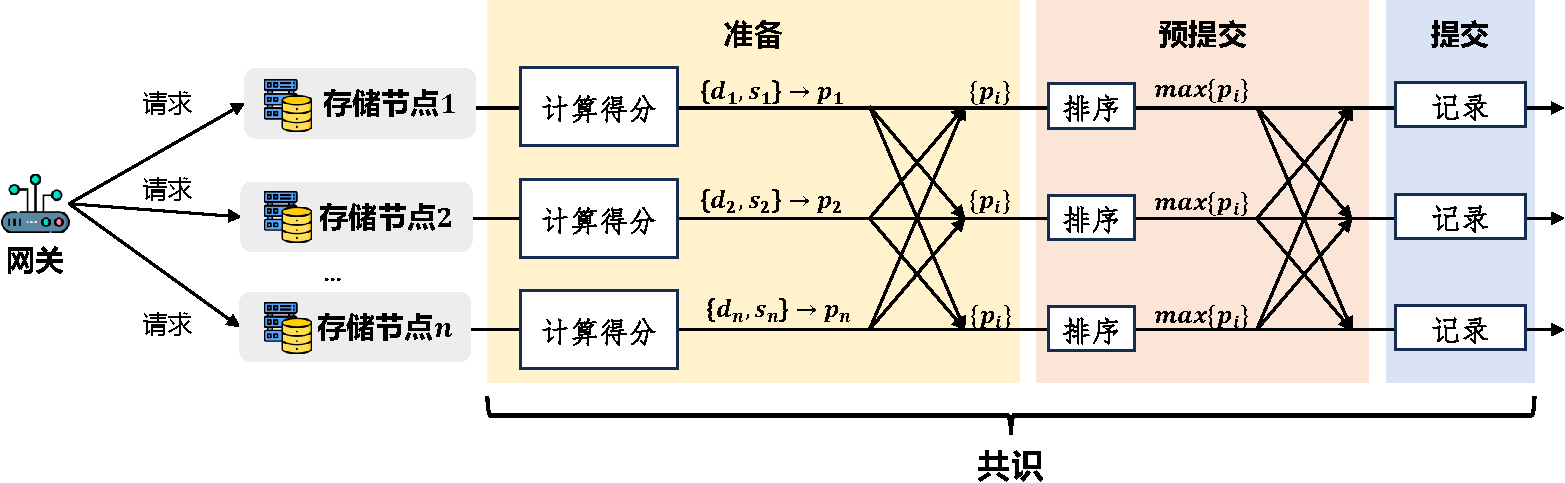
\includegraphics[width=1\linewidth]{timechain/consensus.pdf}
    \caption{基于共识的节点选择机制工作流}
    \label{fig:consensus}
\end{figure}

\begin{algorithm}
	\caption{共识过程}
	\label{algo:consensus}
	\begin{algorithmic}[1]
        \renewcommand{\algorithmicrequire}{ \textbf{Prepare}}
        \REQUIRE
            \STATE $request \gets \textit{receive}(REQUEST)$
            \IF{$request$ is valid}
                \STATE $d_i \gets \textit{distance}(i.pos, request.pos)$
                \STATE $s_i \gets i.space$
                \STATE get $p_i$ with xxx
                \STATE $\textit{broadcast}(p_i, \textit{PREPARE})$
            \ENDIF

        \renewcommand{\algorithmicrequire}{ \textbf{PreCommit}}
        \REQUIRE
            \STATE $\{p_i\} \gets \textit{receive}(\{p_i\}, \textit{PREPARE})$
            \IF{$\textit{count}(\textit{PREPARE}) > 2 * f + 1 \textit{ and timeout}$}
                \STATE $P \gets \max_n \{p_i\}$
                \STATE $\textit{broadcast}(P, \textit{PRECOMMIT})$
            \ENDIF

        \renewcommand{\algorithmicrequire}{ \textbf{Commit}}
        \REQUIRE
            \STATE $P \gets \textit{receive}(P, \textit{PRECOMMIT})$
            \IF{$count(P) > f + 1$}
                \STATE $\textit{commit}(P)$
            \ENDIF
	\end{algorithmic}
\end{algorithm}

为了安全地选择最佳存储节点,TimeChain提出了一种基于共识机制的节点选择算法。
整个选择过程包括\textit{request}、\textit{prepare}、\textit{pre-commit}、\textit{commit}和\textit{reply},其详细信息如~\autoref{fig:consensus}所示,算法如~\autoref{algo:consensus}所示。
与PBFT共识类似,在\textit{request}阶段,网关向系统中的所有节点发送请求,共识节点将在\textit{reply}阶段将获得的结果返回给网关。
同样类似于PBFT共识,我们假设拜占庭卫星的数量为$f$,卫星总数超过$3f+1$。

在\textit{prepare}阶段,每个节点通过考虑存储节点的距离、信誉等来计算分数,并将分数广播给所有其他节点。
我们使用$p_i=\alpha\cdot d_i+\beta\cdot s_i+\gamma\cdot q_i$来计算第$i$个节点的得分,其中$d_i$表示第$i$节点和客户端节点之间的距离,存储服务质量$q_i$可以从链上的服务记录中评估,$s_i$表示节点的剩余存储空间。
所有这些数据都可以在链上找到。
$\alpha$、$\beta$和$\gamma$是加权参数,这些系数可以根据特定的系统需求和性能要求进行调整。

在\textit{pre-commit}阶段,共识节点从其他节点接收准备好的消息集$\{p_i\}$。
当此节点的计时器超时并且收到超过$2f+1$prepare消息时,共识节点根据它们收到的信誉优先级$\{p_i\}$决定最佳存储提供者。
如果每一轮共识只返回最近的节点,由于距离对信誉计算机制的影响,一些较近节点的存储压力可能会非常高。
为了平衡负载,共识节点将返回一组信誉最高的$n$节点,供网关随机选择,而不是信誉最高的节点。

在\textit{commit}阶段,所有节点都将收到其他节点推荐的最佳存储决策。
当相同的预提交消息的数量超过$f+1$时,此节点将向客户端提交最佳存储节点。

\subsection{安全分析}
我们在这里考虑这一共识协议的安全性。
由于TimeChain的共识协议只是基于PBFT添加了额外的信息,我们只考虑\textit{prepare}和\textit{pre-commit}阶段额外信息带来的安全风险。
在\textit{prepare}阶段,如果一个节点伪造了自己的分数,网关可以很容易地检查分数的真实性,因为评估数据源都可以在链上找到。
一旦节点伪造了其信誉,该行为也将被记录在链上,从而影响下一次的信誉评估。
此外,由于最后只选择了一个存储节点,网关不关注所有节点得分的真实性,只关注所选节点的得分。
在\textit{pre-commit}阶段,如果任何节点伪造了最终得分,则不会影响最终结果。
这是因为对于包含$f$拜占庭节点的$3f+1$节点的网络,必须在\textit{commit}阶段获得相同的结果。

\section{基于LSH树的验证机制}
\label{sec:lsh}
为了解决因传输大量验证数据而导致的高网络传输延迟问题,我们提出了一种新的LSH树,并通过尾部合并策略优化其空间。

\subsection{LSH树}

\begin{figure}[t]
    \centering
	\begin{minipage}{0.85\linewidth}
        \centering
        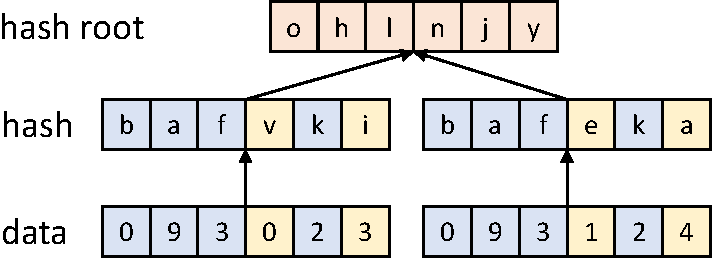
\includegraphics[width=1\linewidth]{timechain/lsh-tree.pdf}
        \caption{LSH树结构}
        \label{fig:lsh_tree}
	\end{minipage}
\end{figure}

对位置敏感的哈希将类似的数据映射到类似的哈希值以进行重复数据删除。
顾名思义,我们通常打包在物理空间或时间上接近的数据,这些数据往往具有很高的局部相似性。
因此,通过在同一批上使用局部敏感哈希,我们可以得到相似的哈希值。
当需要传输哈希值时,只传输哈希差部分,从而减少了要传输的数据量。

我们在~\autoref{fig:lsh_tree}中展示了LSH树的一个例子。
具体来说,对于批处理中的数据,我们采取类似于默克尔树的步骤,首先对原始数据执行局部敏感散列。
对于哈希结果,我们将两个相近的哈希合并为一个字符串,并计算该字符串的局部敏感哈希值。
然后,我们逐层向上重复这个过程,直到我们得到一个唯一的哈希值,即哈希根。
在第一级哈希中,由于原始数据的高度相似性,哈希值的许多位是相同的。
因此,在传输第一级哈希值时,我们只能传输不同的比特以减少传输延迟。
同样,由于第一级哈希中存在局部相似性,第二级哈希中的许多比特也将相似。
通过类比,对于每一层的哈希值,我们只需要传输哈希差比特,从而进一步减少了传输的数据量。

由于我们使用LSH树而不是原始的Merkle树,因此我们需要分析LSH树的安全性。
这里我们主要考虑存储提供者篡改数据的情况,即仍然可以用不同的原始数据获得相同的哈希值的情况。
我们测试了LSH树的不同层,发现在最接近数据源的哈希层中,哈希的平均差位数为170bit。
这已经超过了MD5和SHA1标准,这些标准现在在物联网场景中非常常用~\cite{chi2017hashing,landge2018secured}。
对于靠近根节点的LSH树的层,尽管哈希差位数较少,但这对篡改原始数据没有意义。

\subsection{尾部合并}

\begin{figure}[t]
    \centering
	\begin{minipage}{0.8\linewidth}
        \centering
        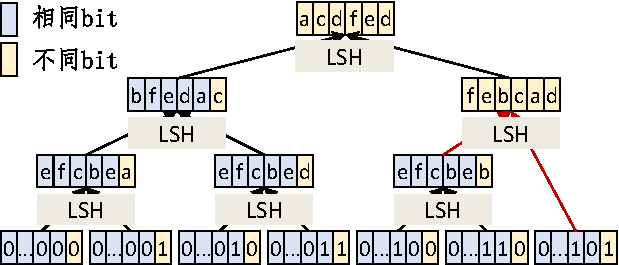
\includegraphics[width=1\textwidth]{timechain/tail_merging_lsh.pdf}
        \caption{非满二叉LSH树}
        \label{fig:tail_merging_lsh}
	\end{minipage}
\end{figure}

\begin{figure}[t]
    \centering
	\begin{minipage}{0.8\linewidth}
        \centering
        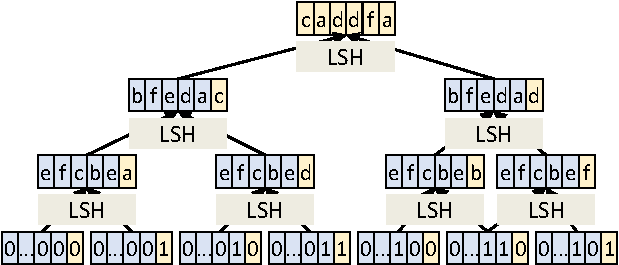
\includegraphics[width=1\textwidth]{timechain/tail_merging_tail.pdf}
	\end{minipage}
	\caption{尾部合并下的非满二叉LSH树.}
	\label{fig:tail_merging_tail}
\end{figure}

在一个完整的二叉树中,LSH-tree可以通过成对地批量合并数据来执行局部敏感哈希。
然而,如果批处理中的数据数量不足以形成完整的二叉树,那么像Merkle树一样构建哈希树将导致相似性的丧失。
例如,在~\autoref{fig:tail_merging_lsh}中,一批中有7个数据点,对于一个完整的二叉树来说,这个大小是不满足的。
在第一轮散列中,前6个数据成对执行LSH。
由于原始数据的相似性,这6个数据的哈希结果是相似的。
在第二轮哈希中,由于数据5-6和第7个原始数据的第一轮哈希结果非常不同,这两个数据的哈希结果也与数据点1-4的哈希结果非常不一样。
在执行完整性证明时,需要传输所有这些不同的散列数据位,这增加了传输的数据量。

为了解决这个问题,我们引入了尾部合并策略,将非全二叉树的尾部节点与同一层的前节点合并。
如图~\autoref{fig:tail_merging_tail}所示,在第一轮哈希中,我们将第7个节点和第6个节点合并,以尽可能保持数据的相似性。
数据6-7的哈希结果是\texttt{efcbeb},数据5-6的哈希值是\texttt{efcbef}。
显然,在第一轮哈希中存在很高的相似性,并且可以保持到下一级哈希。
这将传输的哈希值大小从12位减少到7位,代价是在第一轮哈希中只传输了1个不同的位。
这样,在进行完整性证明时,我们只需要传输不同的哈希位,从而减少了传输的数据量。

\section{性能评价}
在本节中,我们将评估TimeChain的存储性能和查询性能。

\subsection{实验设置}
我们基于一些开源项目(如Hyperledger Fabric和IPFS)实现TimeChain。
块大小设置为1500,块间隔为1秒。
我们模拟了分布在世界各地的320个云服务器节点,并基于该集群进行了实验。
每个存储节点配置2核CPU和4GB内存,每个存储节点的存储空间为512GB。
存储节点和网关之间的距离从800公里到6000公里不等,平均为4000公里。
考虑到一些存储提供商存在欺诈行为,远程存储的数据将无法访问,概率为60\%。
我们使用PC作为物联网传感器的网关节点,它配备了Intel(R)Core i7-13700K CPU@5.4GHz、32GB DRAM,并运行Ubuntu 22.04。
默认批大小和查询大小设置为20。

\subsubsection{基线}
\textbf{SEBDB}~\cite{zhu2019sebdb}是链上数据库的典型代表。
它通过将所有数据存储在区块链上并使用B+树创建时间戳和设备名称的快速索引,实现了对链上区块的高效访问。
在数据验证方面,SEBDB使用传统的Merkle树进行数据验证。
Merkle树通过计算数据块的哈希值并将这些哈希值逐层组织成树结构来实现数据完整性验证。

\textbf{FileDES}~\cite{xu2024filedes}是一个基于文件的存储系统。
它通过在远程节点上存储数据并在链上记录数据的哈希值来实现数据的安全存储和可靠性。
当客户端需要搜索数据时,FileDES会遍历区块链上的所有块,以获取数据的存储位置。
在数据验证方面,FileDES也使用与SEBDB相同的Merkle树。

\subsubsection{数据集和工作负载}
我们使用以下三个数据集:港珠澳大桥(Bridge)~\cite{zhang2023edge}, RT-IFTTT(RT)~\cite{heo2017rt}和天气(WX)~\footnote{https://www.kaggle.com/selfishgene/historical-hourly-weather-data/}。
考虑到时间序列存储系统~\cite{naqvi2017time}的存储特性,我们将数据集中的设备信息附加到传感器值的头部,每条数据占用56B的空间。
我们根据这三个数据集的数据生成率,将这三个数据库的平均数据查询范围分别设置为100、20和10。

\subsection{总体性能}

\begin{figure*}[t]
    \centering
	\begin{minipage}{0.48\linewidth}
        \centering
        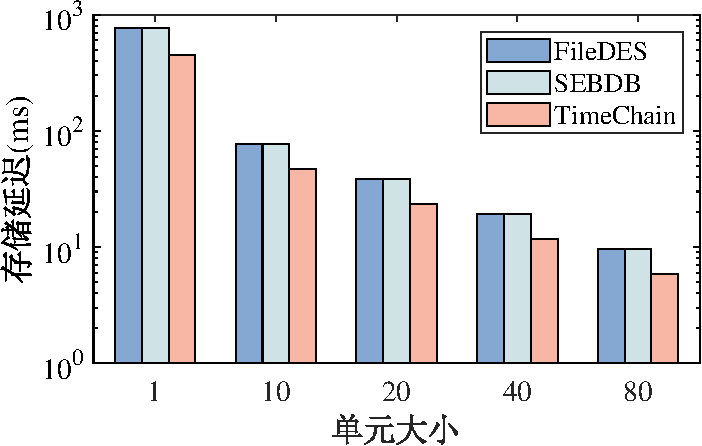
\includegraphics[width=1\textwidth]{timechain/storage_rt_eval.pdf}
        \caption{存储延迟}
        \label{fig:storage_rt_eval}
    \end{minipage}
    \quad
    \begin{minipage}{0.48\linewidth}
        \centering
        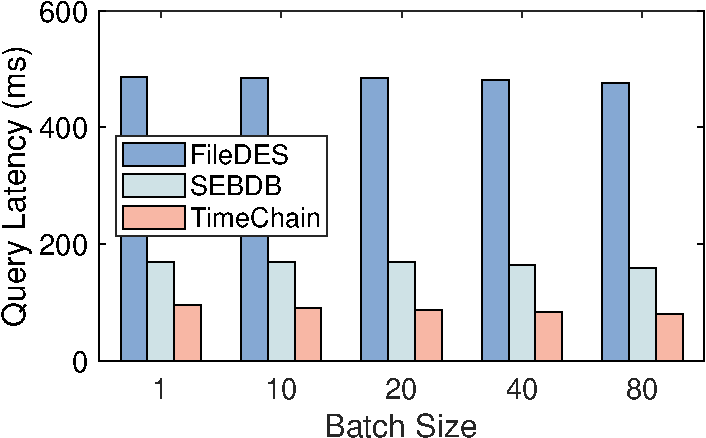
\includegraphics[width=1\textwidth]{timechain/query_rt_eval.pdf}
        \caption{查询延迟}
        \label{fig:query_rt_eval}
	\end{minipage}
\end{figure*}

\textbf{存储延迟。}
我们比较了不同批处理大小下的存储延迟。
由于物联网设备数量众多,数据生成速度快,我们将存储延迟定义为存储10000个数据的总延迟,而不是关注单个数据的微延迟。
如~\autoref{fig:storage_rt_eval}所示,对于不同的批处理大小,TimeChain的存储延迟低于SEBDB和FileDES。
这是因为TimeChain的独特打包机制和节点选择机制减少了数据传输延迟。
此外,随着批大小变大,存储延迟变小。
这是因为,对于相同数量的数据,当批量较大时,数据在链中打包和记录的次数会减少。
用户可以通过调整批处理大小来控制存储延迟。

\textbf{查询延迟。}
我们比较了不同批量大小的查询延迟,如~\autoref{fig:query_rt_eval}所示。
查询延迟是指基于固定查询范围随机查询数据集的平均延迟。
从~\autoref{fig:query_rt_eval}可以看出,TimeChain的查询延迟低于其他两种方案。
这是由于TimeChain减少了数据传输延迟,原因将在~\autoref{fig:query_breakdown}中解释。
我们还可以发现,当批处理大小增加时,查询延迟会减少。
这是因为当批大小增加时,同一查询中涉及的批数量会减少,用户的查询结果将试图集中在一个存储节点上。
然而,批量越大,TimeChain相对于其他解决方案的改进将随着批量的增加而减少。
这是因为当批大小非常大时,相当于将所有数据存储在一个批中,在这种情况下,数据聚类不会导致性能提高。
此外,当大量数据集中在存储节点中时,存储系统的可扩展性和可靠性也会受到损害。

\begin{figure*}[t]
    \centering
    \begin{minipage}{0.48\linewidth}
        \centering
        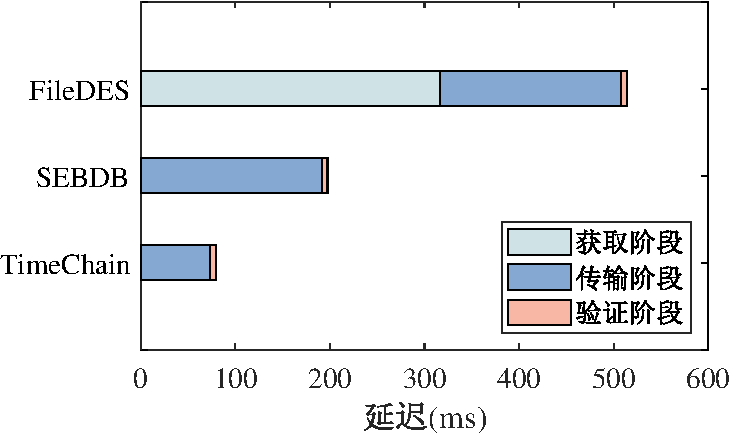
\includegraphics[width=1\linewidth]{timechain/query_breakdown.pdf}
        \caption{查询延迟分解}
        \label{fig:query_breakdown}
	\end{minipage}
	\quad
	\begin{minipage}{0.48\linewidth}
        \centering
        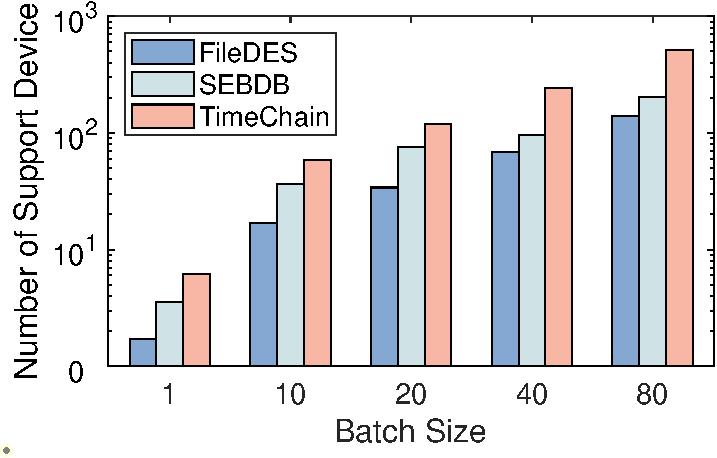
\includegraphics[width=1\linewidth]{timechain/support_device.pdf}
        \caption{最大支持存储设备数}
        \label{fig:support_device}
    \end{minipage}
\end{figure*}

\textbf{查询延迟分解。}
我们进一步分析了查询延迟的细分,如~\autoref{fig:query_breakdown}所示。
查询的延迟主要由4个阶段组成,检索、传输、验证和返回。
考虑到传感器通常选择更近的网关,返回阶段的延迟几乎可以忽略不计。
在验证阶段,三种方案的延迟相对接近,小于1ms,几乎可以忽略不计。
传输和检索阶段的延迟是查询延迟的主要部分。
TimeChain的传输延迟明显低于FileDES和SEBDB。
这是因为TimeChain独特的节点打包机制和选择机制,减少了数据获取次数,缩短了与存储提供商的距离。
对于检索阶段,由于FileDES遍历所有块来检索数据,因此检索延迟特别高。
而SEBDB和TimeChain分别使用B+和R树分别构建索引,从而将延迟降低到1ms以下。

\textbf{支持的最大存储设备数。}
具体来说,我们使用支持设备的最大数量指标,即存储系统每秒可以支持存储服务的设备数量。
我们假设网关可以处理来自多个物联网设备的数据存储请求,并忽略网关本身的处理延迟。
所有物联网设备同时以1hz的频率生成数据,并要求在生成下一个数据之前必须存储这些数据。
如~\autoref{fig:support_device}所示,TimeChain与SEBDB和FileDES相比,支持的最大设备数量分别增加了1.63倍和3.55倍。
这主要是由于TimeChain的快速存储延迟,其中数据传输延迟非常低,允许TimeChain以更快的速度存储数据。
此外,支持的设备的最大数量将随着批量大小的增加而增加。
当批量大小达到80时,TimeChain支持的最大设备数已达到数千。

\begin{figure}[t]
    \centering
	\begin{minipage}{0.45\linewidth}
        \centering
        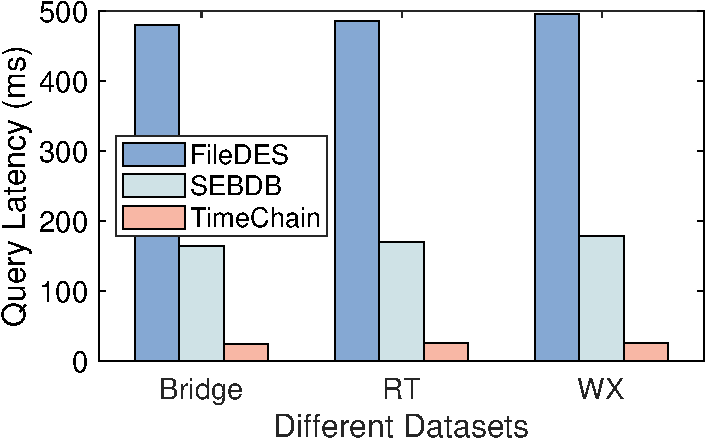
\includegraphics[width=1\textwidth]{timechain/query_diff_dataset.pdf}
        \caption{不同查询大小下的查询延迟}
        \label{fig:query_diff_dataset}
	\end{minipage}
	\quad
	\begin{minipage}{0.45\linewidth}
        \centering
        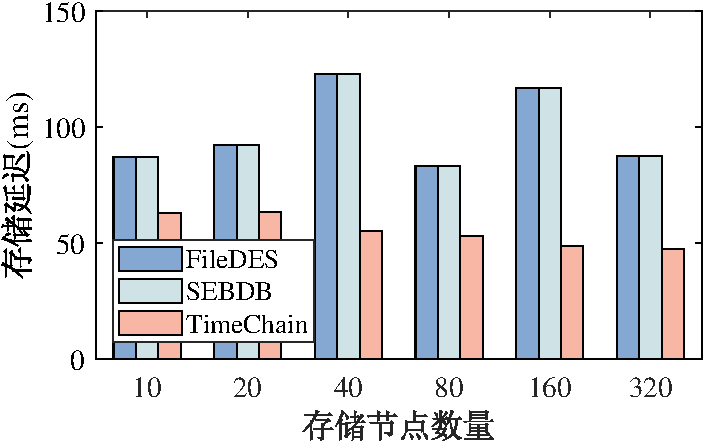
\includegraphics[width=1\textwidth]{timechain/storage_diff_storage_nodes.pdf}
        \caption{不同存储网络下的存储延迟}
        \label{fig:storage_diff_storage_nodes}
    \end{minipage}
\end{figure}

\subsection{不同参数下的性能}
\textbf{不同查询大小下的查询延迟。}
我们比较了三种不同查询大小数据集(Bridge、RT和WX)的查询性能,结果如~\autoref{fig:query_diff_dataset}所示。
三个数据集中工作负载的平均查询大小分别为10、20和40。
我们可以发现,这三种解决方案的查询延迟通常随着查询大小的增加而降低。
这可以归因于这样一个事实,即更大的查询大小意味着查询中覆盖了更多的数据,从而提高了数据局部性和查询效率。
我们观察到,与SEBDB和FileDES相比,当查询大小变大时,TimeChain带来的性能改进也会增加。
这是因为当查询大小变大时,SEBDB和FileDES通常需要从比TimeChain更多的节点获取数据。

\textbf{存储网络规模下的存储延迟。}
我们比较了不同存储网络规模下每种解决方案的存储延迟,如~\autoref{fig:storage_diff_storage_nodes}所示。
随着存储节点数量的增加,TimeChain的存储延迟呈下降趋势。
这是因为当节点数量增加时,TimeChain中的网关可以选择更多的存储提供程序,这增加了选择更近节点的可能性。
其他解决方案将不会从存储节点数量的增加中受益。
这是因为FileDES和SEBDB都随机选择存储节点,而不断增长的存储节点不会显著影响随机选择的结果。
因此,FileDES和SEBDB的存储延迟显示出相对较大的随机性。

\subsection{消融实验}
在本小节中,我们通过三项消融研究证明了我们的设计的改进效果。

\begin{figure*}[t]
    \centering
	\begin{minipage}{0.8\linewidth}
        \subfloat[查询延迟]{
            \centering
            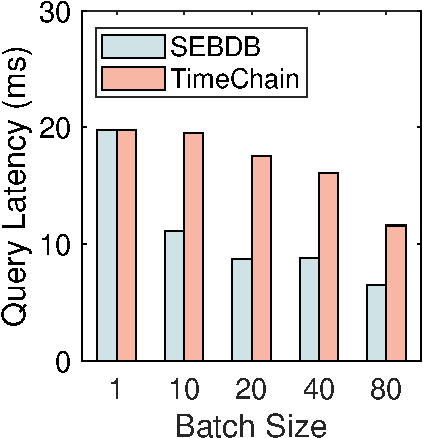
\includegraphics[width=0.45\textwidth]{timechain/ratiocut_latency_eval.pdf}
            \label{fig:ratiocut_latency_eval}
        }
        \subfloat[跨越的batch]{
            \centering
            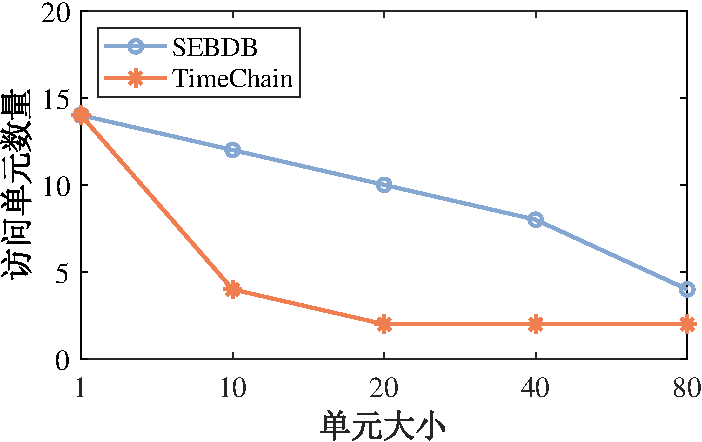
\includegraphics[width=0.47\textwidth]{timechain/ratiocut_batch_eval.pdf}
            \label{fig:ratiocut_batch_eval}
        }
        \caption{聚类算法消融实验} 
    \end{minipage}
\end{figure*}

\textbf{聚类算法。}
我们比较了聚类算法的效果,并将TimeChain与SEBDB进行了比较。
如~\autoref{fig:ratiocut_latency_eval}所示,与SEBDB相比,TimeChain的网络传输延迟减少了40.3\%。
SEBDB中的打包节点没有考虑用户查询的规律性,聚合数据也没有根据数据源的类型进行划分。
当数据所有者请求一系列数据时,SEBDB网关需要跨越来自更多存储提供商的多个批次。
TimeChain使用光谱聚类算法根据用户请求的特征对来自特定传感器的数据进行打包,导致访问批次比SEBDB少59.3\%,如~\autoref{fig:ratiocut_batch_eval}所示。

\begin{figure*}[t]
    \centering
    \begin{minipage}{0.8\linewidth}
        \vspace{0.5ex}
        \subfloat[查询延迟]{
            \centering
            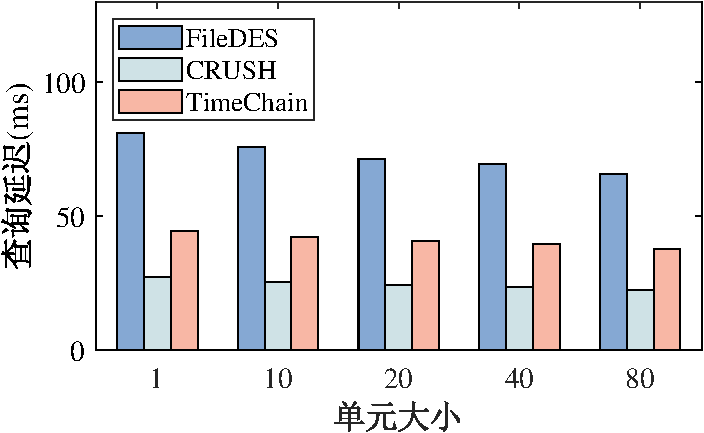
\includegraphics[width=0.45\textwidth]{timechain/consensus_latency_eval.pdf}
            \label{fig:consensus_latency_eval}
        }
        \subfloat[存储服务质量]{
            \centering
            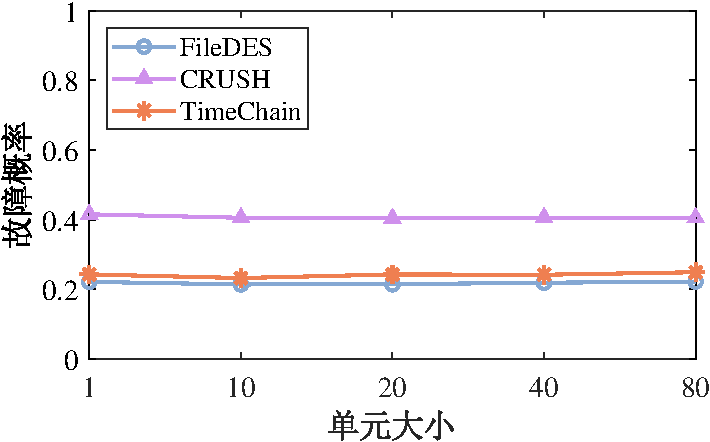
\includegraphics[width=0.47\textwidth]{timechain/consensus_prob_eval.pdf}
            \label{fig:consensus_prob_eval}
        }
        \caption{节点选择消融实验} 
    \end{minipage}
\end{figure*}

\textbf{节点选择。}
我们在~\autoref{fig:consensus_latency_eval}中显示了TimeChain、FileDES和CRUSH在节点选择方面的性能差异。
FileDES~\cite{xu2024filedes}根据节点信誉划分一些受信任的存储节点,并从节点集中随机选择节点来存储数据。
因此,FileDES在三者中具有最高的存储服务提供概率,如~\autoref{fig:consensus_prob_eval}所示。
然而,FileDES的随机节点选择可能会引入更远的存储节点,从而导致更长的传输延迟。
CRUSH~\cite{weil2006ceph}根据节点的物理位置选择最近的节点进行存储,但不考虑存储节点故障和单点故障。
这使得CRUSH可以选择更接近但不可靠的存储节点,因此CRUSH选择的41\%的节点无法提供有效的存储服务。
另一方面,TimeChain考虑了节点的物理距离和节点信誉,在响应时间和服务概率方面都具有最佳性能。
虽然TimeChain选择的节点距离不是最接近的,但考虑到节点距离和服务质量,TimeChain的效果最好。

\begin{figure*}[t]
    \centering
    \begin{minipage}{0.8\linewidth}
        \vspace{-0.5ex}
        \subfloat[查询延迟]{
            \centering
            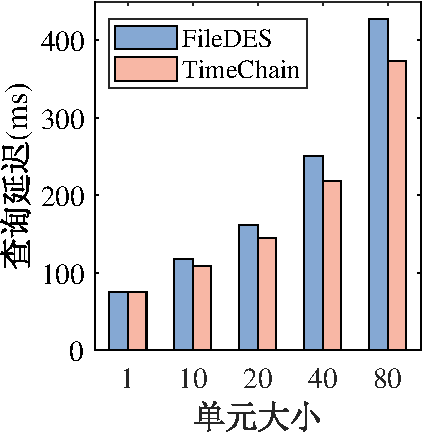
\includegraphics[width=0.45\textwidth]{timechain/lsh_latency_eval.pdf}
            \label{fig:lsh_latency_eval}
        }
        \subfloat[完整性证明大小]{
            \centering
            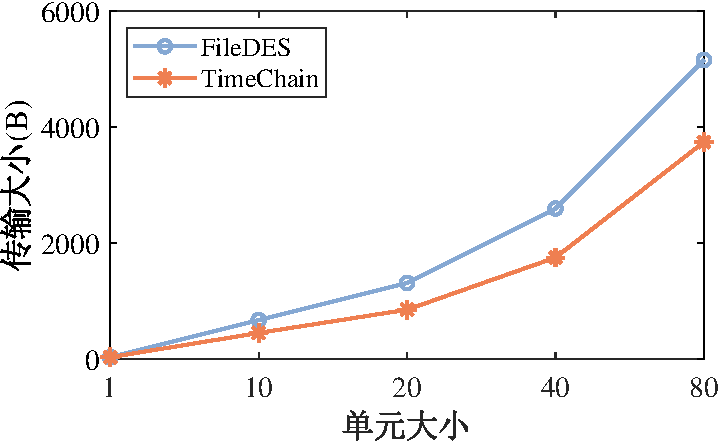
\includegraphics[width=0.47\textwidth]{timechain/lsh_size_eval.pdf}
            \label{fig:lsh_size_eval}
        }
        \caption{LSH树消融实验} 
    \end{minipage}
\end{figure*}

\textbf{LSH树。}
我们比较了FileDES和TimeChain的网络传输延迟,如~\autoref{fig:lsh_latency_eval}所示。
与FileDES相比,TimeChain的数据传输延迟减少了10.9\%。
这是由于当局域网中有更多的传感器设备并且数据生成频率很高时,数据传输量会显著影响拥塞网络中的传输延迟。
如~\autoref{fig:lsh_size_eval}所示,由于TimeChain使用lsh作为哈希算法,通过网络传输的数据量大大减少。
这将减少存储和查询延迟,并大大减轻存储提供商的存储负担。

\section{本章小结}

\chapter{基于距离度量的移动区块链算存一体化激励机制}
\section{移动区块链的交互过程}
\section{基于斯塔克伯格博弈的交互模型}
\section{纳什均衡分析}
\section{实现与评估}
\section{本章小结}

\chapter{总结与展望}
